\section{SONUÇLAR}

%\subsection{Genel Açıklamalar}


\begin{comment}
Sonuçlar bölümü yapılan çalışmada varılmak istenen hedefe ulaşılıp
ulaşılmadığını gösteren çıktıları ve bunların açıklamalarını
içermelidir. Pratik ya da deneysel çalışmanın fotoğrafı sonuç değildir.
Sonuç, o çalışmanın yapılma amacına göre çalışıp çalışmadığını gösteren
grafik, rakam, çizelge vb çıktılardır. Yani sayısal değerler ya da
görsel grafiklerdir. Eğer bir motor hız kontrolü yapıyorsanız, bunun
sonucu motorun fotoğrafı değil, o motorun verdiğiniz referans hızlarda
çalışıp çalışmadığını gösteren hız-zaman grafikleridir. Eğer RF tabanlı
bir iletişim projesi yapmışsanız, bunun sonucu da RF devresinin
fotoğrafı değil, açık yada engelli alanlarda ne kadar mesafeden
haberleşmeyi sağlayabildiğini gösteren ölçüm sonuçlarına ait çizelge
veya grafiklerdir. Sonuçların gösterildiği bütün şekil, grafik ve
çizelgelere metin içerisinde atıfta bulunulmalı ve gerekli açıklamaları
yapılmalıdır.

\textbf{Grafiklerin eksenleri birimleriyle birlikte mutlaka
yazılmalıdır. Grafik formatı için Mühendislik Tasarımı veya Bitirme
Projesi Yazım Kılavuzuna bakınız.}

Sonuçlar bölümünün muhtemel alt başlıkları aşağıdaki gibi olabilir.

\subsection{6.2. Simülasyon Sonuçları}

Mühendislik Tasarımı kapsamında yapılan simülasyon çalışmalarının
sonuçları bu altbaşlıkta yer alır. Elde edilen veriler, çizelge veya
grafikler ile verilerek tasarlanan sistemin hedeflenen amaçları sağlayıp
sağlamadığı açıklanmalıdır. Simülasyon sonuçları yorumlanarak deneysel
çalışmalardan beklentiler verilmelidir.

\subsection{6.3. Deney Sonuçları}

Yapılan pratik çalışmalardan elde edilen test ve ölçüm sonuçları bu alt
başlıkta verilerek tasarlanan sistemin hedeflenen amaçları sağlayıp
sağlamadığı açıklanmalıdır. Deneysel sonuçlar simülasyon sonuçları ile
karşılaştırılarak birbirleriyle olan benzerlik ve farklılıkları
açıklanmalı, varsa farklılıkların nedenleri anlatılmalıdır.
\textbf{Yapılan sistemin fotoğrafı sonuç değildir.} Böyle bir fotoğraf
konulabilir. Fakat bu sonuç değildir. \textbf{Sonuç o sistemin yapılma
nedenini sağlayıp sağlamadığının gösterilmesidir.} Bu nedenle testler
yapılarak elde edilen sayısal veriler grafiklerle ve çizelgelerle
açıklanmalı ve tartışılmalıdır.
\end{comment}




\subsection{Genel Açıklamalar}
Bu çalışmada amaçlanan hedefe ulaşılma durumu, elde edilen sayısal sonuçlar ve görsel grafiklerle ortaya konmuştur. Elde edilen çıktılar, çalışmanın amacına uygunluğu ve doğruluğu açısından değerlendirilmiştir. Aşağıda sunulan grafikler, sistemin performansını farklı parametreler ve koşullar altında göstermektedir.

\begin{figure}[H]
    \centering
    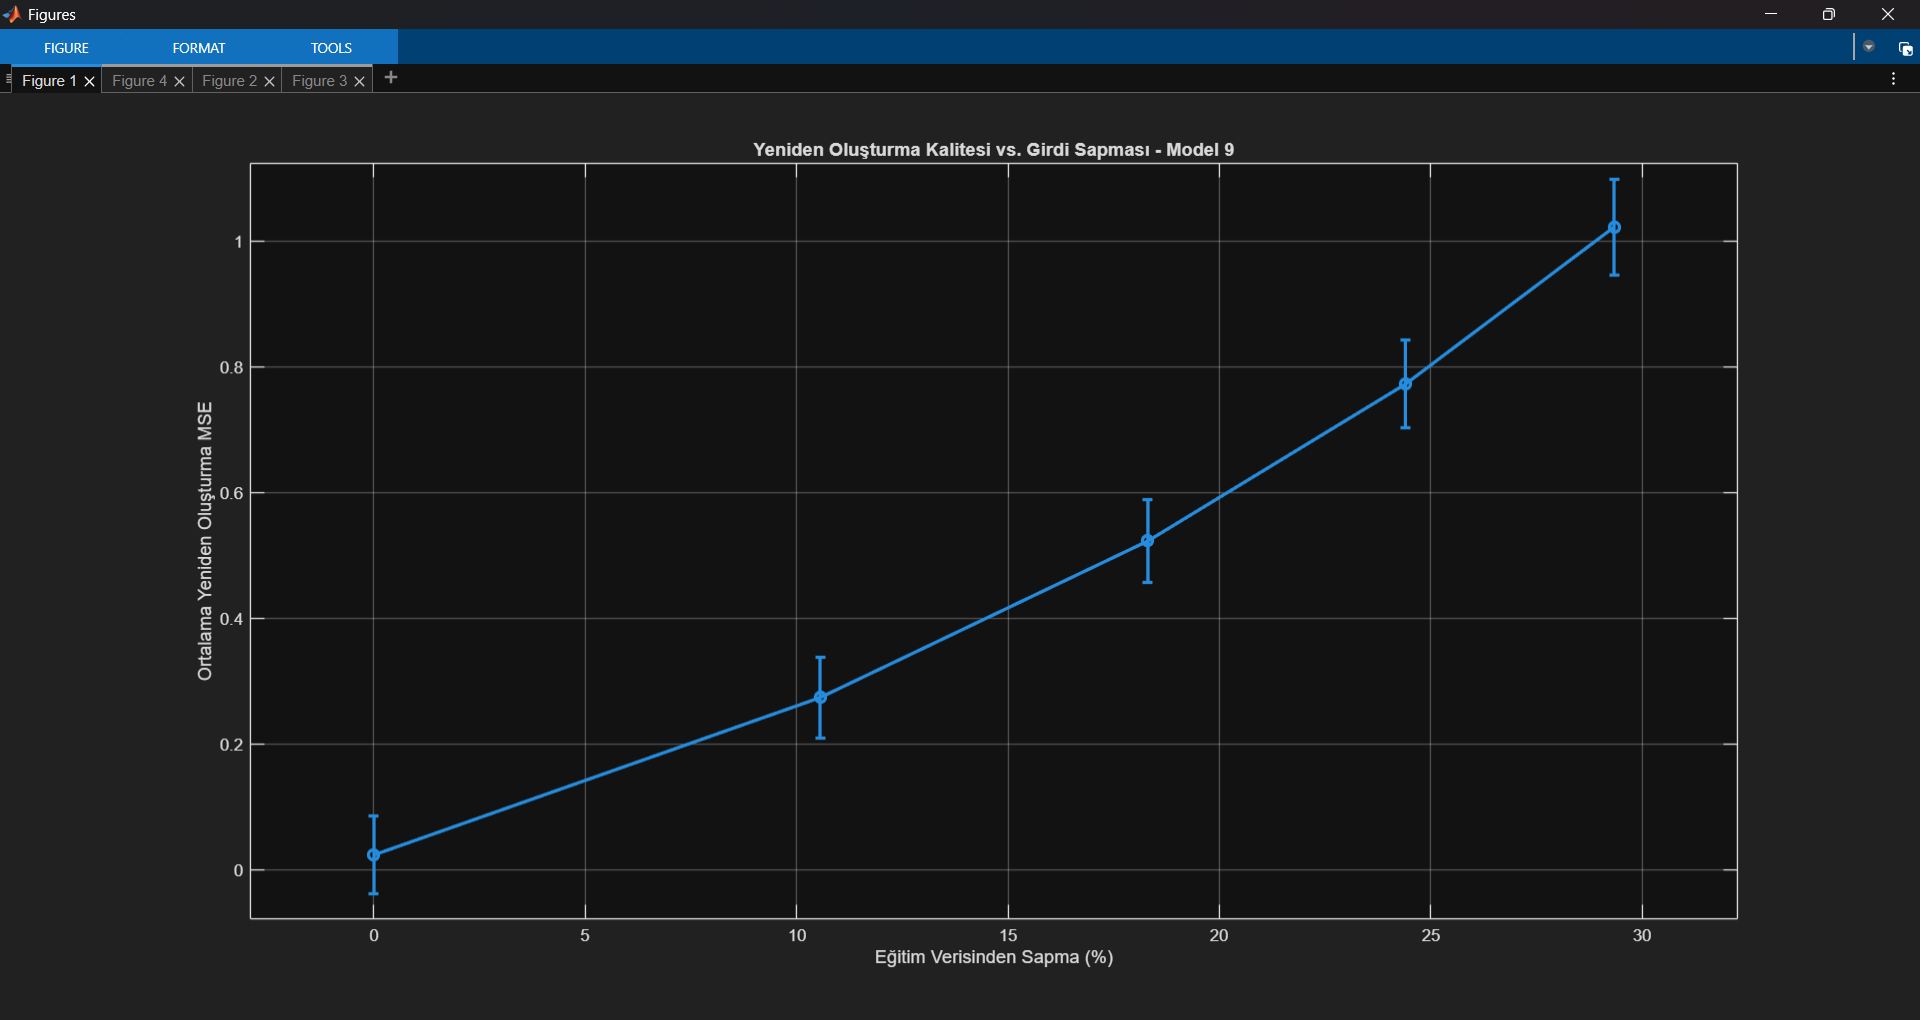
\includegraphics[width=1\linewidth]{image_sonsim.png}
    \caption{Eğitim verisinden sapma ile ortalama yeniden yapılandırma hatası (MSE) arasındaki ilişki}
    \label{fig:sonsim1}
\end{figure}

\subsection{Simülasyon Sonuçları}
Bu bölümde, geliştirilen konvolüsyonel otomatik kodlayıcı tabanlı modelin simülasyon sonuçları ayrıntılı olarak sunulmaktadır. Simülasyonların temel amacı, modelin öğrenme kabiliyeti, yeniden oluşturma başarımı ve genelleme performansını farklı gürültü seviyeleri altında değerlendirmektir. Ayrıca, öğrenilen temsillerin veri kümeleri üzerindeki ayrıştırma gücü ve sınıflandırma potansiyeli de incelenmiştir.

İlk olarak, her biri 1000 örnek uzunluğunda olan zaman serisi verileri Z-skora göre normalize edilmiş ve \%75 eğitim, \%25 doğrulama olacak şekilde ayrılmıştır. Eğitim verisine belirli sinyal-gürültü oranlarına (SNR) karşılık gelen yapay Gauss gürültüsü eklenerek veri artırımı uygulanmıştır. Bu süreçte -5 dB ile 30 dB arasında değişen 60 farklı SNR seviyesine göre 3000 farklı sinyal üzerinde toplam 180.000 örnek oluşturulmuştur.

Model eğitimi için farklı gizli temsile (latent dimension) sahip 40 farklı konvolüsyonel otomatik kodlayıcı mimarisi denenmiş, her biri için ortalama kare hata (MSE) ve doğrulama kaybı izlenmiştir. Her modelin doğrulama başarımı ve parametre sayısı analiz edilerek, boyut–başarım dengesi gözetilmiştir. Bu amaçla normalleştirilmiş doğrulama kaybı ve model büyüklüğü (parametre sayısı) birleştirilerek en uygun mimari seçilmiştir.



\subsubsection{Eğitim Verisinden Sapma (\%) – Ortalama Yeniden İnşa MSE İlişkisi}
Simülasyon sonuçlarının ilk bölümünde, modelin yeniden yapılandırma kalitesinin, gürültü seviyesine bağlı olarak nasıl değiştiği analiz edilmiştir. Bunun için orijinal sinyal ile gürültülü sinyal arasındaki Pearson korelasyon katsayısı kullanılarak “Eğitim Verisinden Sapma (\%)” metriği tanımlanmış, bu metrik ile yeniden inşa MSE’si arasındaki ilişki \ref{fig:sonsim1} de gösterilmiştir.


Bu analiz sonucunda, düşük sapma seviyelerinde (yüksek korelasyonlu girişler) modelin yeniden yapılandırma hatasının düşük kaldığı, ancak sapma arttıkça yeniden inşa hatasında belirgin bir yükselme olduğu gözlemlenmiştir. Bu durum, modelin eğitim sırasında öğrendiği temsillerin, aşırı bozulmuş verilere karşı sınırlı esnekliğe sahip olduğunu ortaya koymaktadır.


\subsubsection{Gürültü ve Korelasyonun Test Verisindeki Etkisi}
Her sinyal için farklı gürültü seviyelerinde elde edilen SNR değerleri ve karşılık gelen Pearson korelasyonları görsel olarak analiz edilmiştir. Sinyal-gürültü kombinasyonlarının yeniden yapılandırma kalitesi üzerindeki etkisi \ref{fig:sonsim2}de gözükmektedir.

\begin{figure}[H]
    \centering
    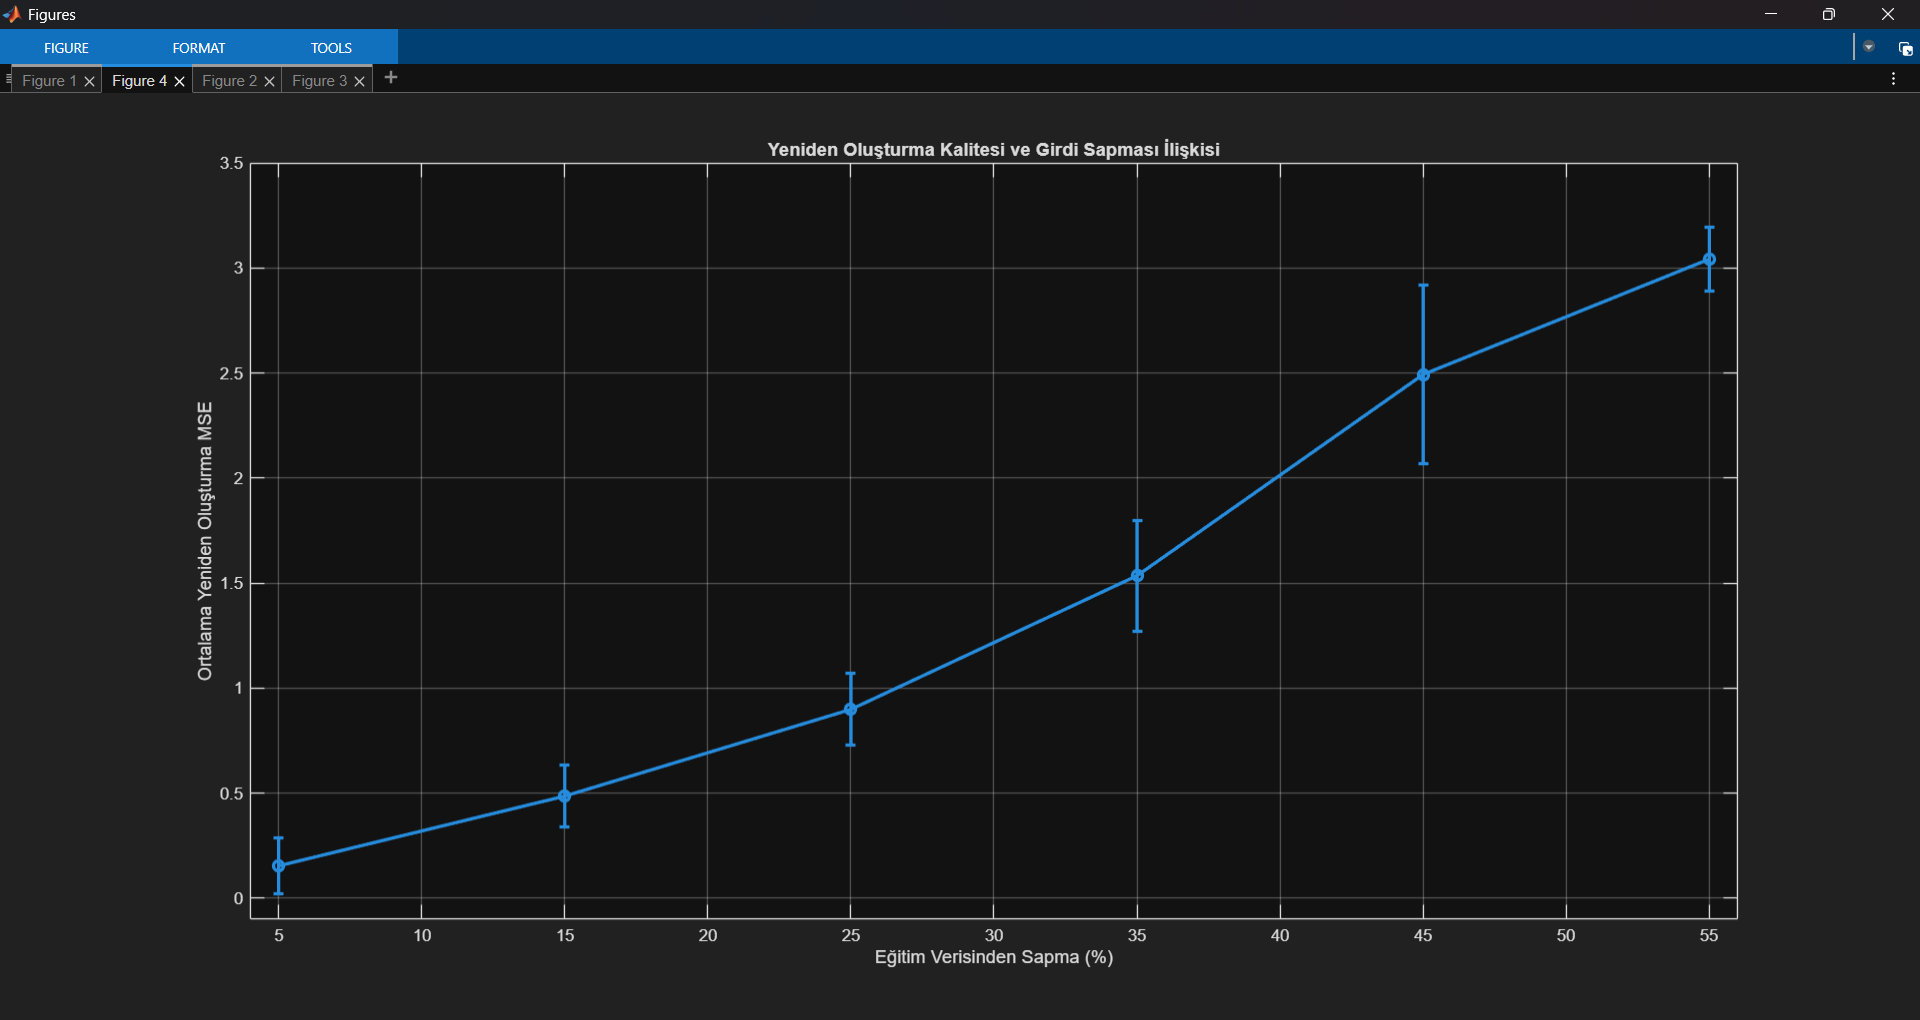
\includegraphics[width=1\linewidth]{image2_sonsim.png}
    \caption{Test verisinin eğitim verisinden sapma ile ortalama yeniden yapılandırma hatası (MSE) arasındaki ilişki}
    \label{fig:sonsim2}
\end{figure}


Bu, modelin sinyal yoğunluğu ve gürültü etkisine olan duyarlılığını değerlendirmede önemli bir araç olmuştur.

\subsubsection{Eşik Yüzeyli 3B Saçılım Grafiği}
Sinyal indeksi, uygulanan SNR değeri ve yeniden yapılandırma hatasının üç boyutlu saçılım grafiği \ref{fig:sonsim3}, sistemin performansını daha geniş bir bakışla ortaya koymaktadır. Renk skalası, her bir gürültü seviyesinde sinyal ile bozulmuş sinyal arasındaki korelasyonu temsil etmektedir.

\begin{figure}[H]
    \centering
    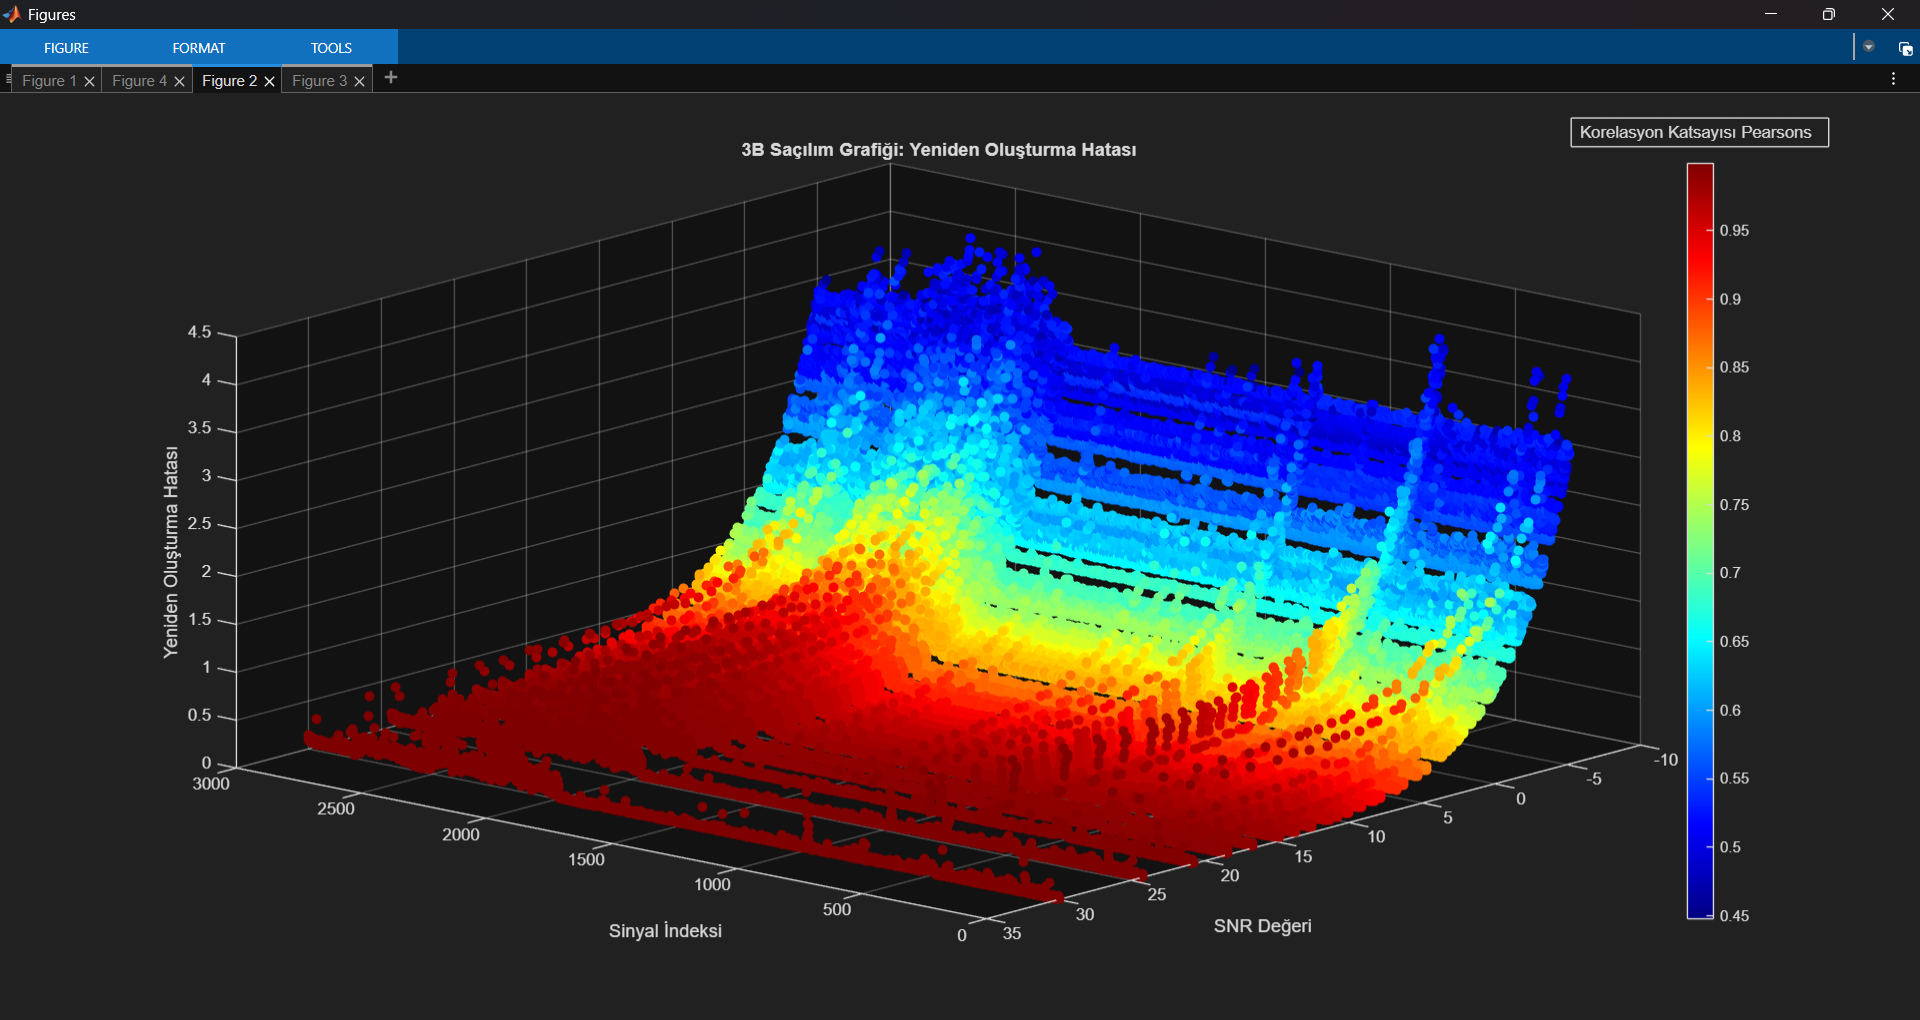
\includegraphics[width=1\linewidth]{image3_sonsim.png}
    \caption{Sinyal İndeksi, SNR ve Yeniden İnşa Hatası arasındaki ilişkiyi gösteren 3B saçılım grafiği.}
    \label{fig:sonsim3}
\end{figure}


Bu görsel analiz, sistemin genel hassasiyetini ve gürültüye karşı dayanımını daha sezgisel biçimde göstermiştir.

\subsubsection{Kümeleme Tabanlı Sınıflandırma Analizi}
Modelin eğitim sonrasında öğrendiği gizli temsiller (latent vektörler) üzerinde K-Means algoritması ile kümeleme yapılmış, ardından bu kümeler ile veri etiketleri arasındaki tutarlılık incelenmiştir. Elde edilen belirsizlik matrisi \ref{fig:sonsim4}, her bir veri segmentinin hangi kümeye atandığını ve modelin ayırt edici gücünü göstermektedir. \ref{fig:sonsim4}de sınıf 1 Engin, sınıf 2 İdris, sınıf 3 Engin veya İdris değil anlamına gelmektedir.



Bu analiz, modelin yalnızca yeniden yapılandırma başarımıyla değil, aynı zamanda sınıflandırmaya yönelik temsiller üretme yetkinliğiyle de etkili olduğunu ortaya koymuştur.




\subsection{Deney Sonuçları}

Deneyde kullanılan program \ref{fig:deney}de görülmektedir.


Projenin deney aşamasında, sistemimizin önünden \textbf{her biri farklı birey olan 3 kişi, ayrı ayrı 100 defa geçerek} toplam 300 gerçek hareket senaryosu oluşturulmuştur. Bu testlerden elde edilen sonuçlar belirsizlik matrisi ile değerlendirilmiştir.

\begin{figure}[H]
    \centering
    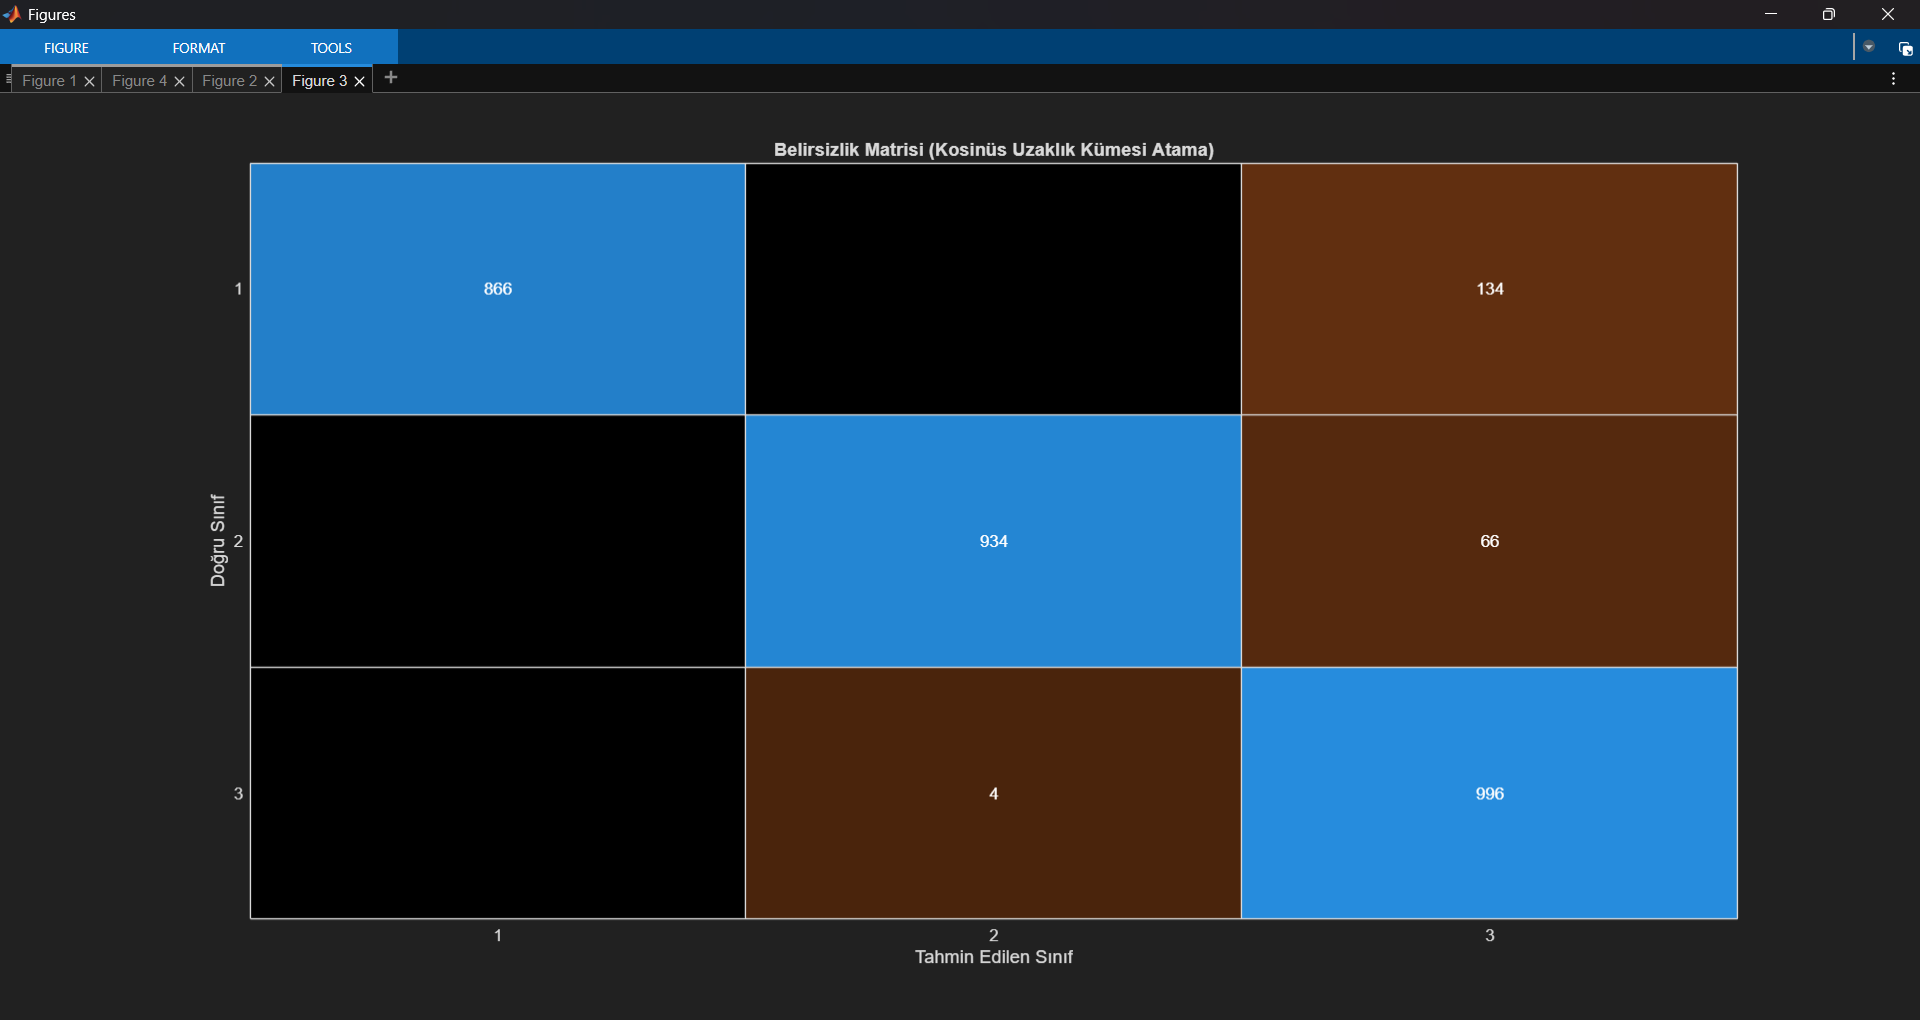
\includegraphics[width=1\linewidth]{image4_sonsim4.png}
    \caption{Kosinüs benzerliğine dayalı kümeleme sonuçlarını gösteren belirsizlik matrisi.}
    \label{fig:sonsim4}
\end{figure}

\begin{itemize}
    \item \textbf{Doğru pozitif:} Modelin gerçek hareketleri doğru algılama oranı yaklaşık \%90'dır.
    \item \textbf{Yanlış pozitif:} Hatalı algılama oranı \%10 civarındadır.
    \item \textbf{Doğru negatif} ve \textbf{yanlış negatif} değerleri de matriste yer almakta olup, bu sayede hassasiyet ve doğruluk hesaplanmıştır.
\end{itemize}

Deneylerde elde edilen belirsizlik matrisi \ref{fig:deney_cm}’de sunulmuştur ve modelin gerçek ortamda da yüksek performans gösterdiğini ortaya koymuştur.


\subsection{Simülasyon ve Deney Belirsizlik Matrislerinin Karşılaştırılması}

Simülasyon ortamında elde edilen belirsizlik matrisi ile gerçek ortamda yapılan testlerden elde edilen deney belirsizlik matrisi ile karşılaştırıldığında; genel olarak benzer doğruluk ve sınıflar arası ayrıştırma eğilimleri gözlemlenmiştir.


Simülasyonda hatalı sınıf atamaları oldukça düşüktür ve doğruluk çok yüksektir; örneğin, 1. sınıf için 866 doğru sınıflama ve sadece 134 hata, 3. sınıf için ise 996 doğru sınıflama ve yalnızca 4 hata bulunmaktadır.


Gerçek deneyde ise toplam 300 örnek üzerinden yaklaşık \%90 doğruluk elde edilmiş; örneğin, 1. sınıfta 100 örneğin 80’i doğru tahmin edilirken, 20’si yanlış tahmin edilmiştir. Deney matrisinde, özellikle 1. sınıfın 2. ve 3. sınıfa karışma oranı simülasyona göre daha yüksektir; bu durum, gerçek ortamda ışık değişkenliğinden kaynaklandığını düşünüyoruz.


Sonuç olarak, simülasyon ve deney sonuçları genel eğilim açısından tutarlıdır; model temel hedefini sağlamış ve sınıflar arası ayrım yapabilmiştir. Ancak deney ortamında ek gürültü ve donanımsal kısıtlar nedeniyle hatalı tahmin oranı artmıştır. Gelecekte sensör çeşitliliğinin artırılması ve haberleşme protokolünün iyileştirilmesi ile deney doğruluğunun simülasyondaki seviyelere yaklaşması beklenmektedir.


\begin{figure}[H]
    \centering
    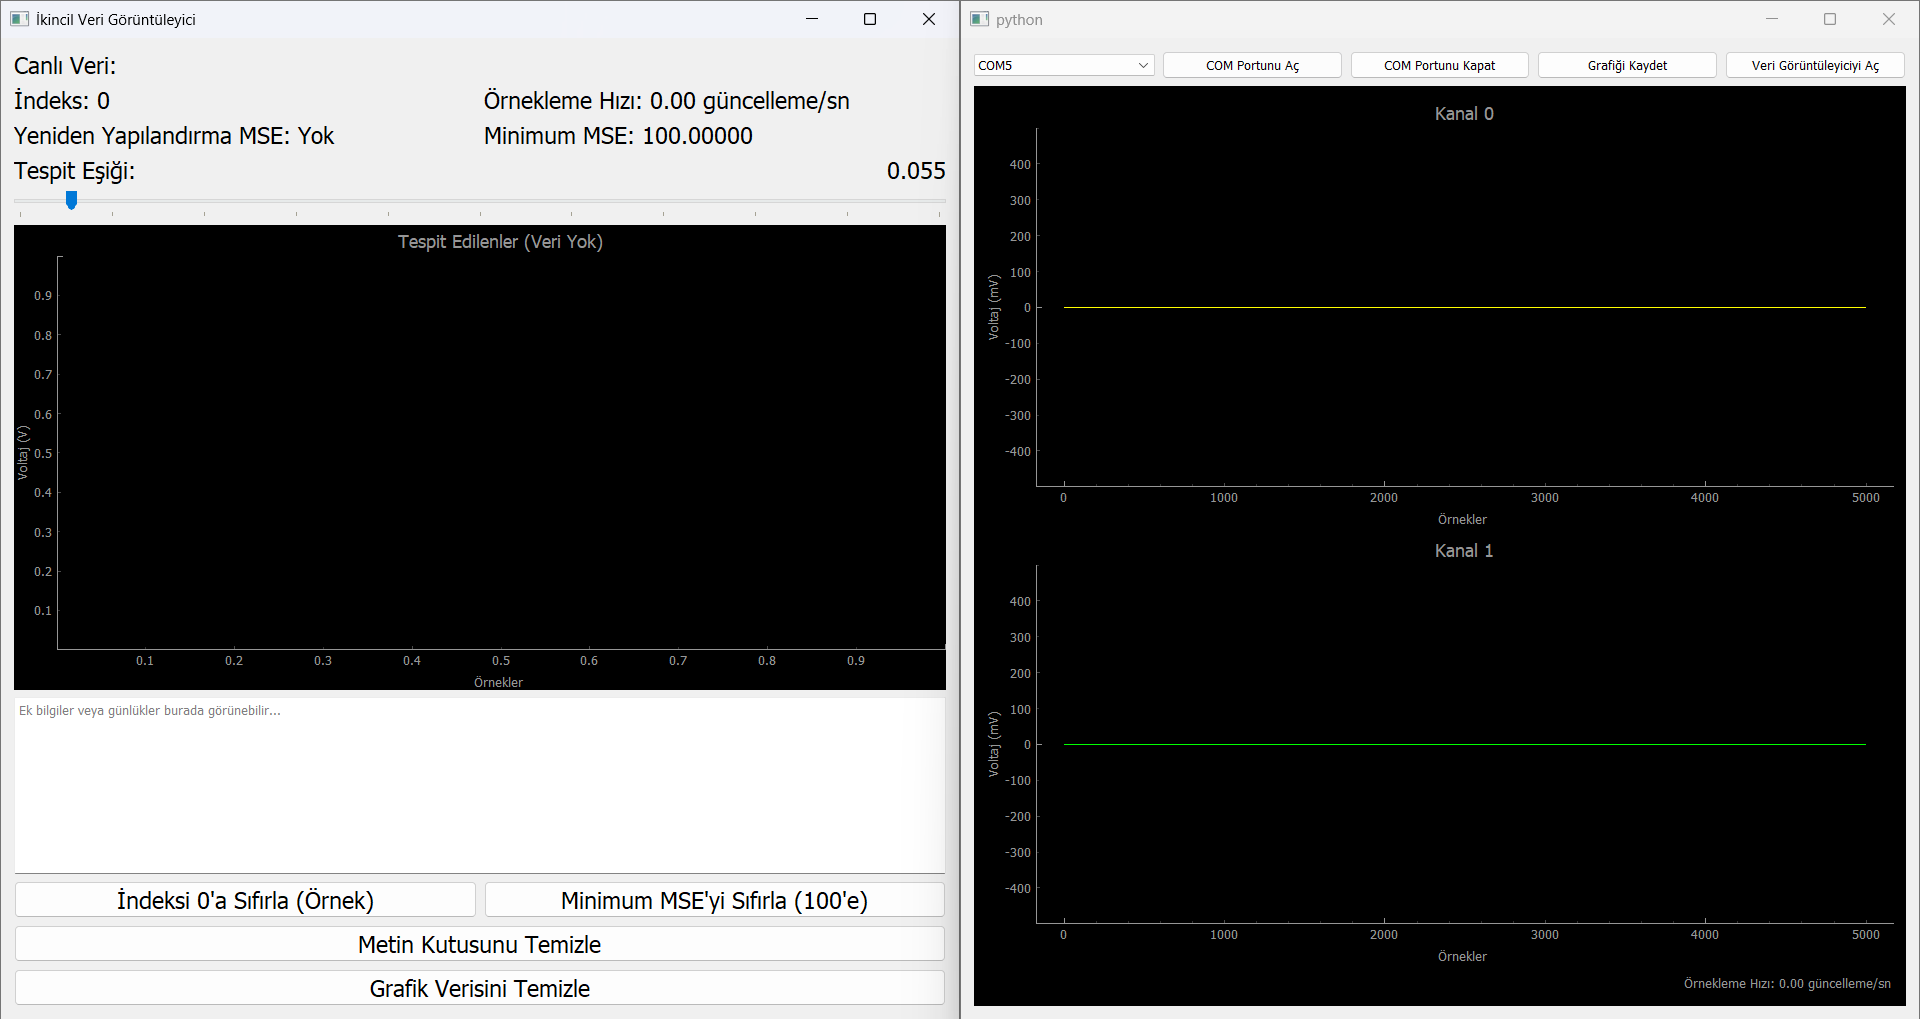
\includegraphics[width=1\linewidth]{media/image_deney.png}
    \caption{Deney Programı}
    \label{fig:deney}
\end{figure}


\subsection{Başka Proje ile Karşılaştırılması}

Bu projede geliştirilen model, Danışman hocamız Prof. İsmail KAYA'nın önerisi ile bitkinin yaprağından alınan voltaj verileriyle test edilmiştir. Bu testlerde model yeniden eğitilmiş, ancak parametreler (katman sayısı, nöron sayısı vb.) bitki verisine uygun şekilde değiştirilmiştir. Bitki verisinde sadece iki sınıf bulunmaktadır:
\begin{itemize}
    \item \textbf{1. sınıf (hareket yok)}: Bitkinin doğal durumu, yani önünden kimse geçmiyor.
    \item \textbf{2. sınıf (hareket var)}: Bitkinin önünden bir kişinin geçmesi.
\end{itemize}

Simülasyon ortamında ise üç sınıf vardır: Engin, İdris ve Taha. Burada Engin ve İdris sınıfları \textbf{hareket var} durumunu, Taha sınıfı ise \textbf{hareket yok} durumunu temsil etmektedir. Bu şekilde sınıflar aşağıdaki gibi eşleştirilmiştir:
\begin{center}
\begin{tabular}{ccc}
\toprule
\textbf{Simülasyon Sınıfı} & \textbf{Gerçek Anlamı} & \textbf{Bitki Verisi Sınıfı} \\
\midrule
1 (Engin) & Hareket var & 2 \\
2 (İdris) & Hareket var & 2 \\
3 (Taha) & Hareket yok & 1 \\
\bottomrule
\end{tabular}
\end{center}



Bitki verisinde elde edilen belirsizlik matrisi \ref{fig:bitki_cm}de görünmektedir.
\begin{itemize}
    \item Gerçek hareket yok durumunda 983,429 doğru negatif tahmin ve 5 yanlış pozitif tahmin.
    \item Gerçek hareket var durumunda 147 doğru pozitif tahmin ve 9 yanlış negatif tahmin.
\end{itemize}


\textbf{Karşılaştırma ve yorum:}
\begin{itemize}
    \item Simülasyon ortamında hatalı tahmin oranı görece yüksektir; örneğin 1. ve 2. sınıflarda (hareket var) 134 ve 66 hata, 3. sınıfta (hareket yok) sadece 4 hata bulunmaktadır.
    \item Bitki verisinde ise hareket yok durumunda çok büyük miktarda veri (983,429 örnek) üzerinde test yapılmış ve sadece 5 hatalı pozitif tahmin yapılmıştır. Hareket var sınıfında ise 147 doğru tespit ve sadece 9 yanlış negatif vardır.
    \item Bu sonuç, bitki verisinde modelin özellikle hareket olmayan durumları çok yüksek doğrulukla (neredeyse hatasız) tespit edebildiğini göstermektedir. Ancak hareket var sınıfında sınırlı sayıda örnek olması nedeniyle doğruluk simülasyona göre daha düşüktür.
\end{itemize}

\begin{figure}[H]
    \centering
    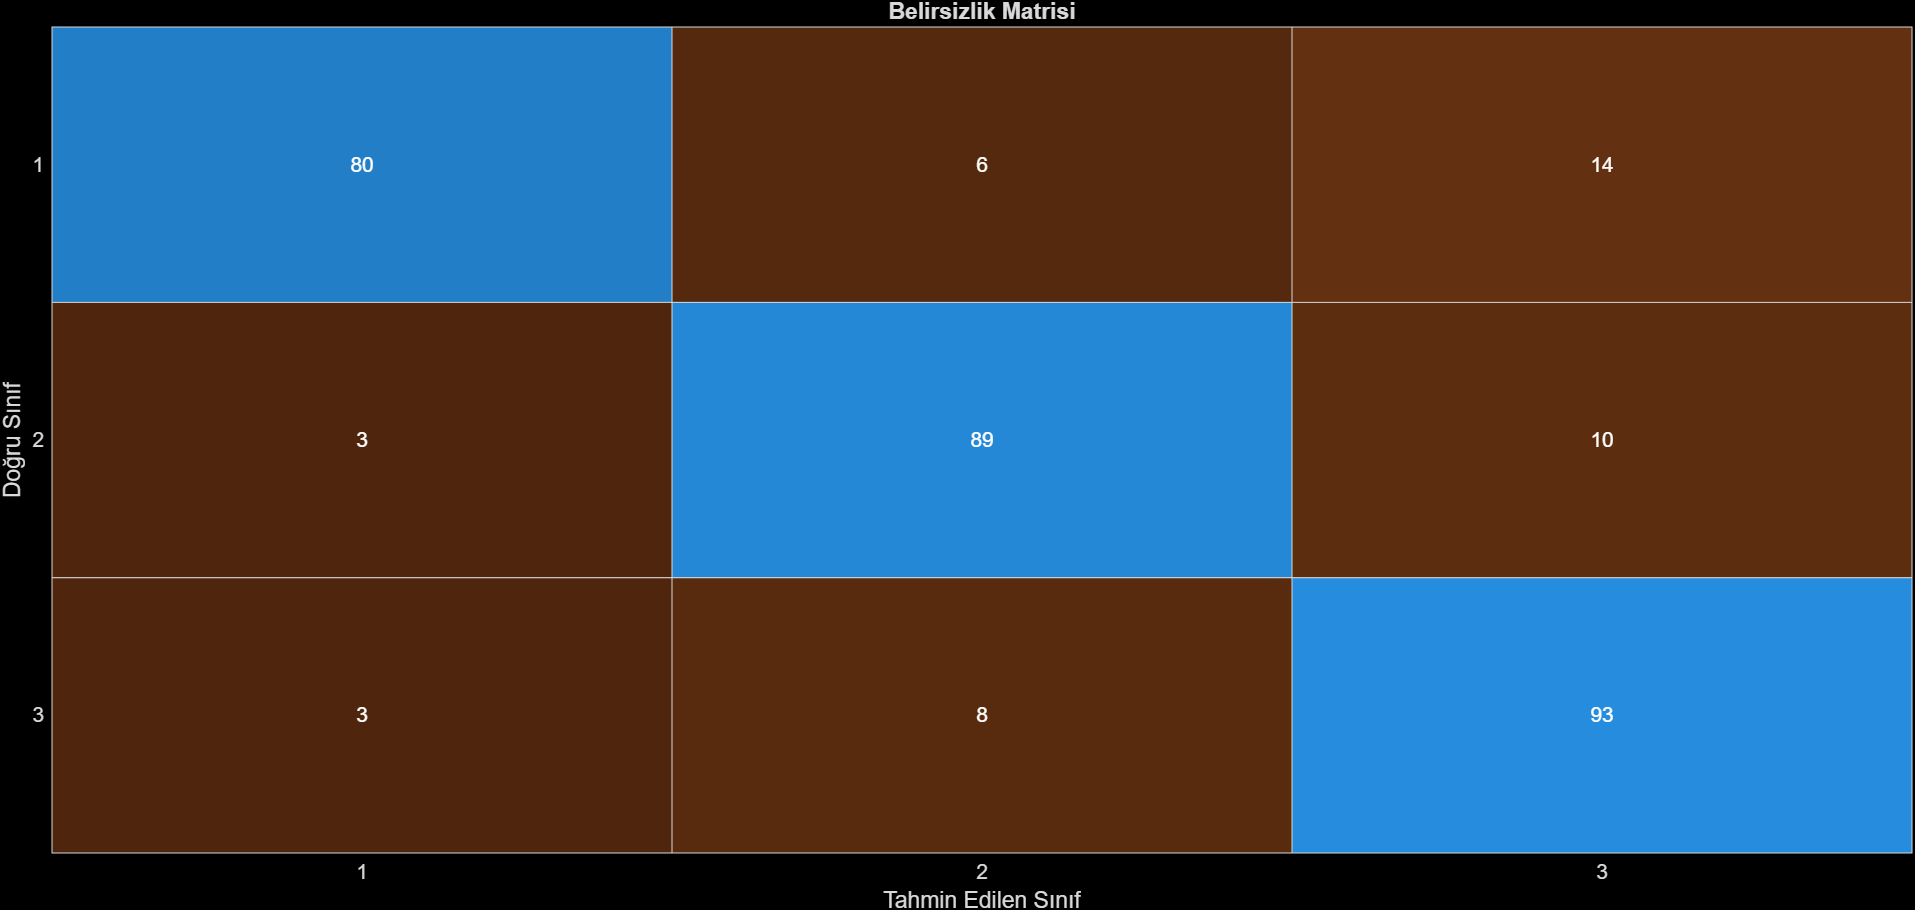
\includegraphics[width=1\linewidth]{image_deney_cm.png}
    \caption{Gerçek ortamda 3 kişiyle yapılan testlerden elde edilen belirsizlik matrisi.}
    \label{fig:deney_cm}
\end{figure}

Sonuç olarak, simülasyon ortamında model sınıflar arası ayrıştırmayı genel olarak başarılı şekilde yaparken; bitki verisinde, çok daha dengesiz ve gerçekçi verilerle test edilmesine rağmen hareket yok durumunu neredeyse mükemmel ayırt edebilmiş, hareket var durumunda ise sınırlı veri nedeniyle kısmen daha düşük başarı göstermiştir. Bu, modelin güçlü negatif algılama (hareket yok) kabiliyeti olduğunu; ancak gerçek ortamda pozitif sınıf sayısını artırarak (örneğin farklı hareket senaryolarıyla) genel doğruluğun daha da iyileştirilebileceğini göstermektedir.


\begin{figure}[H]
    \centering
    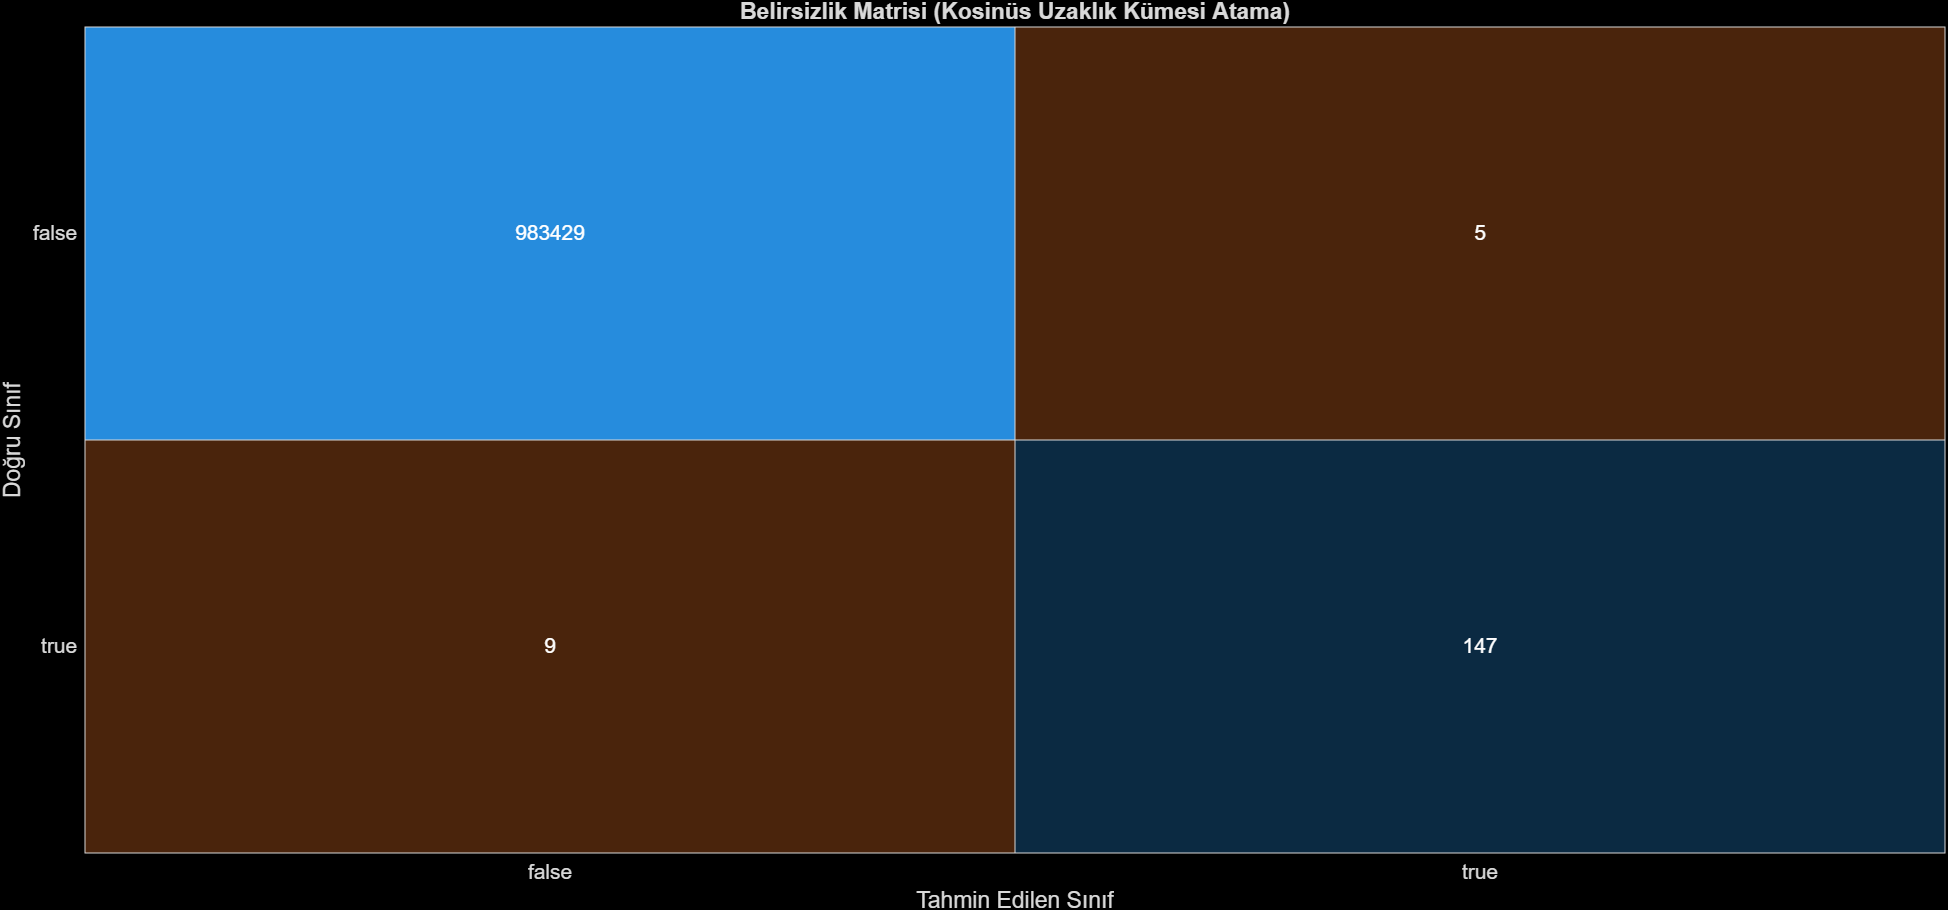
\includegraphics[width=1\linewidth]{image_bitki.png}
    \caption{Bitkinin yaprağından alınan voltaj verileriyle test edilen modelin belirsizlik matrisi}
    \label{fig:bitki_cm}
\end{figure}


